\documentclass[../../main.tex]{subfiles}

\begin{document}
    

\section{Audio}
Steganography in audio is more challenging with respect to images, because
the \emph{human auditory system} (HAS) operates over a wide dynamic range,
while maintaining a high sensitivity to perturbations and noises.
Howerer, there are still some ``holes'' where data can be hidden.
The HAS has a quite small differential range, so loud sounds mask out quiet
sounds, moreover it is unable to perceive absolute sound phase, but only
relative one.

Another important factor to consider when dealing with sound are the
transmissions enviroments.
Audio signals can be transmitted through a digital channel (eventually being
resampled), through an analog channel or ``over the air'' played by a
speaker and received by a microphone.
Depending on the transmission channel there could be huge modification that
can make the steganalysis process impossible, but also that can compromise
irreparably the hidden message, damaging also the steganographer
\cite{techniques-data-hiding}.

In the following sections we will cover some of the possible ways in which
steganography and steganalysis is applied in audio signals.

\subsection{Non-compressed and compressed methods}
We can distinguish two different types of audio steganography: steganography
on \emph{non-compressed} audio files and on \emph{compressed} ones.
The first ones aims at exploiting the vulnerabilities of the \emph{HAS}
presented above, whereas the second ones perform minor modifications to
embedd data based on the way in which the compression is perfomed
\cite{review-audio-steganalysis}.

\subsection{Phase coding}
The phase encoding method works by modifying the \emph{absolute phase} of
audio signals to convey information, while maintaining the \emph{relative
phase} in order to not compromise imperceptibility.

\subsubsection{Encoding procedure}
Firstly the sound is sampled into \emph{N} short segments. To each one of them 
a \emph{discrete Fourier transform} (DFT) is applied, constructing two matrices: $\phi_n(\omega)$ for the phase 
and  $A_n(\omega)$ for the magnitude. Sequently the phase difference between ajacent segments is stored and the message to hide 
is converted into a phase message, representing with $\frac{\pi}{2}$ or $-\frac{\pi}{2}$ respectively 0 or 1.
The phase matrix is then recomputed by embedding the message into it. Finally the original message is reconstructed applying an inverse DFT.

\subsubsection{Steganalysis techniques}
The steganalysis techniques for phase coding system follows a
procedure similar to the encoding ones, since is based on a statistical
analysis of \emph{phase discontinuites}, but which requires the use of a
classification algorithm in order to distinguish between natural and
modified signals.

As proposed in \cite{steganalysis-phase-coding}, the signal is divided into segments to which is applied a
\emph{fast Fourier transform} (FFT) in order to extract the phase difference between adjacent segments.
Such phase difference is then monitored, calculating statistical features of the sample. Finally a \emph{SVM classifier} (support-vector machines) is used to
 detect if the signal has been modified or not.

A SVM classifier, after a proper training, is able to clearly distinguish
between elements by mapping them into two different classes by means of
linear regression and statistical calculus.
This method is applied varying the length of segements to which the FFT is
applied.

\subsection{Echo embedding methods}
The echo embedding methhods hide data introduzing or varying an \emph{eco}.
\begin{figure}[h]
    \centering
    \caption{Echo kernels and parameters}
    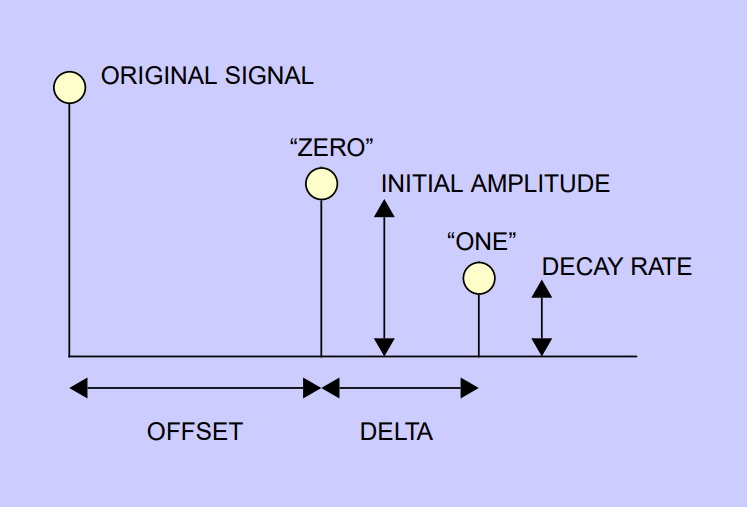
\includegraphics[scale=0.6]{audio_echo.png}
\end{figure}
Data are hidden by varying \emph{initial amplitude}, \emph{decay rate} and
\emph{offset}.
\subsubsection{Encoding}
Encoding procedure is performed by dividing the signal into smaller
portions and the echoing each portion as an independent signals by an audio
mixing process.
The coder use two different delay times to represent a binary zero(offset)
and a binary one(offset+delta), both below audible threshold, considering
the initial amplitude and that the decay rate follows and exponential
behaviour.
The final signal is formed by recombining all independent encoded signal
portions.
The transitions between one and zero are done by slightly modify the zero
and one kernel in order to maximize imperceptibility.
\subsubsection{Steganalysis}
The steganalysis process of echo encoded signals is done by doing a
statistical analysis on the \emph{cepstrum}, which is the result of the
Fourier transform on the decibel spectrum of the signal.
As presented in \cite{review-audio-steganalysis}, the cepstrum is calculated
in a sample window possibly smaller than the encoding segment length.
The sampling window is moved over the length of the signal and the cepstrum
recomputed each time.
Then, the results can be analyzed by classifying every sampled cepstrum in
one of four possible categories:
\begin{itemize}[noitemsep]
    \item Inside a zero embedded segment
    \item Inside a one embedded segment
    \item Crossing from a one(zero) to a zero(one)
    \item Crossing from a one(zero) to a one(zero)
\end{itemize}
This classification is possible due to the fact that the cepstrum plotting
exhibits peaks when encountering a delay defined by the 0 or 1 kernels.
Moreover, cepstrum peak location aggregation rate (CPLAR) is introduced as
the ratio between detected peaks and number of sampled windows.
CPLAR is used to discriminate between natural and steganographed audio
signals.
This method is also capable of detecting the length of the segmentation
used by the coder.

\subsection{Mp3 steganalysis}
The last type of audio steganalysis that we will briefly treat regards the
\emph{Mp3} format, which is one of the most used compressed sound formats,
since it provides a high compression rate and a good quality.

The Mp3 compression algorithm consist of two nested loops.
The \emph{inner loop} does the quantization of the data and determines the
suitable quantizer step in function of the available quantity of bits.
Whereas the \emph{outer loop} controls the distorsion of the encoding and
keeps it beyond the percpetion level.

The most common steganographic algorithms apply some modifications on the
encoding algorithm, for instance, modify the termination condition on the
inner loop and hide the data during the compression process or modify the
compression coefficients or parameters saved (for instance by replacing the
LSB).

To perform a steganalystic process on an Mp3 file is necessary to do a
statistical analysis on the lenght of the quantization steps or on the
\emph{MDCT} (modified discrete cosine transform) coefficients, the transform
used in the compression algorithm.
The analysis methods are similar to ones presented in the other sections in
this paper, since they rely on some previous knowledge of what is expected
and on calculations that will tell if there is or not a message encrypted.

\end{document}